\newpage
\setcounter{figure}{0}
\setcounter{table}{0}
\setcounter{equation}{0}
\renewcommand{\thefigure}{A\arabic{figure}}
\renewcommand{\thetable}{A\arabic{table}}
\renewcommand{\theequation}{A\arabic{equation}}

\section{Supplementary Information}

Supplementary Information: Quantum Synthetic Data Generation for Industrial Bioprocess Monitoring

\textbf{Table of Contents}\\
A.1 Comparison of Synthetic Data Generation Approaches\\
A.2 Extended Background on GANs and Quantum Computing\\
A.3 Hybrid-GAN Framework for Future Work\\
A.4 Additional Validation Metrics Discussion\\
A.5 Code and Data Availability\\
A.6 Additional Figures\\
A.7 Data Transformation Details\\
A.8 Critic Network Architecture Details

\subsection{Comparison of Synthetic Data Generation Approaches}

\begin{table*}
\footnotesize
  \caption{Approaches for Bioprocess Synthetic Data Generation}
  \label{tbl:bioprocess_methods}
  \begin{tabularx}{\textwidth}{@{}lXXX@{}}
    \toprule
    \textbf{Approach} & \textbf{Description} & \textbf{Advantages} & \textbf{Limitations}\\
    \midrule
    Mechanistic Model-Based & 
    First-principles models simulate bioprocess dynamics under various conditions \cite{vidossich2021role, banga2025mechanistic} & 
    Ensures physical consistency & 
    Limited by model accuracy, understanding of pathways/interactions, and ability to capture process variability \\
    \midrule
    Statistical & 
    Gaussian Process regression and multivariate statistical models generate data based on estimated probability distributions \cite{kim2023, miletic2025utility} & 
    Excel at reproducing statistical properties & 
    Struggle with complex temporal dependencies and rare events \\
    \midrule
    Data-Driven & 
    Machine learning models (VAEs, GANs) learn directly from available data \cite{goodfellow2014generativeadversarialnetworks, akkem2024comprehensive} & 
    Flexible generation without requiring mechanistic understanding & 
    Performance depends heavily on training data quality and quantity \\
    \midrule
    Hybrid & 
    Combine mechanistic knowledge with data-driven techniques \cite{albino2024hybridmodel} & 
    Incorporates physical constraints and biological relationships & 
    Complexity in implementation and model integration \\
    \bottomrule
  \end{tabularx}
\end{table*}

Table~\ref{tbl:bioprocess_methods} summarizes the principal approaches to synthetic bioprocess data generation
discussed in Section~1.2 of the main text. The table highlights the trade-offs between
physical consistency, flexibility, and data requirements across mechanistic, statistical,
data-driven, and hybrid approaches.

\subsection{Extended Background on GANs and Quantum Computing}

 \subsubsection{Classical GAN Architecture}

\begin{figure*}
    \centering
    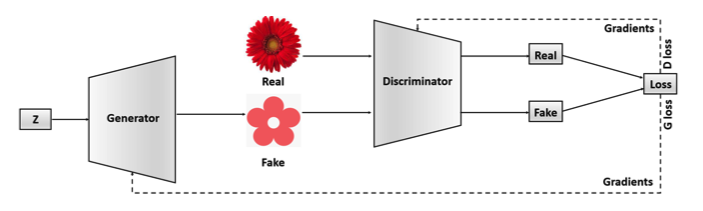
\includegraphics[width=1\linewidth]{classicalgan.png}
    \caption{Illustration of classical GAN architecture.}
    \label{fig:classical_gan}
\end{figure*}

The original GAN formulation by Goodfellow et al. (2014) introduced several key innovations \cite{goodfellow2014generativeadversarialnetworks}: Adversarial training paradigm, Non-cooperative game theory framework, Gradient-based optimization for both networks

\textbf{Training Challenges:}

As discussed in Section~2.1, classical GANs face training instability, mode collapse,
and difficulty with complex multimodal distributions when applied to bioprocess data
\cite{Arjovsky2017, gulrajani2017improved}. These challenges motivate the quantum-enhanced
approach developed in this work.

Specific challenges include:
\begin{itemize}[nosep, leftmargin=*]
  \item \textbf{Mode collapse:} Generator produces limited diversity~\cite{Arjovsky2017}
  \item \textbf{Vanishing gradients:} Discriminator becomes too strong~\cite{goodfellow2014generativeadversarialnetworks}
  \item \textbf{Hyperparameter sensitivity:} Learning rates, batch sizes critically affect convergence~\cite{gulrajani2017improved}
\end{itemize}

\subsubsection{Wasserstein Distance Mathematical Derivation}

The Wasserstein distance, also known as the Earth Mover's Distance (EMD), provides a principled way to measure the dissimilarity between two probability distributions. \cite{villani2008optimal} For two probability measures $\mu $ and $\nu$ on a metric space M with distance function d:
\begin{equation}
    W_p(\mu, \nu) = \left(\inf_{\gamma \in \Gamma(\mu,\nu)} \int_{M \times M} d(x,y)^p d\gamma(x,y)\right)^{1/p}
\end{equation}


where $\Gamma(\mu, \nu)$ denotes the set of all joint probability measures on $M \times M$ with marginals $\mu$ and $\nu$.

\textbf{Kantorovich-Rubinstein Duality:}

For $p=1$, the Wasserstein distance can be expressed as:
\begin{equation}
W_1(\mu, \nu) = \sup_{\|f\|_L \leq 1} \left|\int f d\mu - \int f d\nu\right|
\end{equation}
where the supremum is over all 1-Lipschitz functions.

This formulation allows WGAN to use a neural network (the critic) to approximate the supremum, leading to the practical WGAN objective. \cite{arjovsky17a} The Wasserstein GAN (WGAN) was introduced to address training instabilities by using the Earth Mover's distance to provide a more meaningful and stable loss metric. \cite{arjovsky17a}  The WGAN-GP further refined this approach by replacing weight clipping with a soft gradient constraint. \cite{gulrajani2017improved}

\subsubsection{Quantum Computing Fundamentals for QGANs}

\textbf{Quantum State Representation:}

A quantum state of n qubits is represented by a vector in a $2^n$-dimensional Hilbert space:

$$|\psi\rangle = \sum_{i=0}^{2^n-1} \alpha_i |i\rangle$$

where $\sum_i |\alpha_i|^2 = 1$ (normalization condition).



\textbf{Key Quantum Gates Used:}
\begin{itemize}[nosep, leftmargin=*]
  \item \textbf{Hadamard ($H$):} Creates superposition: $H\ket{0} = \frac{1}{\sqrt{2}}(\ket{0} + \ket{1})$
  \item \textbf{Rotation gates ($R_x$, $R_y$, $R_z$):} Parameterized single-qubit rotations
  \item \textbf{CNOT:} Two-qubit entangling gate
\end{itemize}

\textbf{Quantum Advantage for Generative Models:}

QGANs leverage the inherent properties of quantum systems to provide potential advantages over classical generative models. \cite{Dallaire_Demers_2018, Lloyd_2018, Zoufal_2019}

Specific advantages include:
\begin{itemize}[nosep, leftmargin=*]
  \item \textbf{Exponential state space:} $n$ qubits represent $2^n$ amplitudes, enabling more efficient representation of complex probability distributions \cite{zoufal2021generativequantummachinelearning}
  \item \textbf{Quantum interference:} Constructive/destructive interference explores solution space more efficiently
  \item \textbf{Entanglement:} Creates correlations impossible in classical probability, potentially affecting convergence behaviour; we do not claim a mode-collapse advantage and did not measure one  \cite{romero2019variationalquantumgeneratorsgenerative, Amin_2018}
\end{itemize}

Quantum interference effects can enhance the model's ability to capture subtle correlations and nonlinear relationships present in real-world data, making them particularly suited for complex temporal dependencies found in bioprocess systems. Practical scalability nonetheless remains constrained by current NISQ-device noise and limited circuit depth \cite{Cerezo_2021}.  % [55]-[57],[59] (VQE / option-pricing / QAOA / adversarial-robustness) removed: they do not support a quantum-advantage-for-bioprocess-generation claim (R1-m1)

Recent experimental implementations have demonstrated proof-of-concept QGANs on noisy intermediate-scale quantum (NISQ) devices.  \cite{rudolph2022generationhighresolutionhandwrittendigits, Huang_2021} Rudolph et al. demonstrated that QGANs can generate high-resolution images using an ion trap quantum computer, highlighting the potential of quantum models to exceed classical limitations in certain generative tasks. \cite{rudolph2022generationhighresolutionhandwrittendigits}

\subsection{Proposed Extension (Outlook): Hybrid-GAN-Mechanistic Framework}

\subsubsection{Proposed Mathematical Formulation (not implemented in this study)}

\emph{The following Hybrid-GAN-mechanistic structure is a proposed extension and was not implemented, trained, or evaluated in this work; it is included to motivate future research and is presented as a formulation only.} The proposed Hybrid-GAN-mechanistic structure would integrate generative adversarial networks with physics-informed mechanistic components to enhance predictive modeling in data-scarce environments. This approach complements hybrid machine learning approaches prevalent in chemical and biological process modeling applications, particularly when data availability is limited.  \cite{mansouri2025models, nielsen2020hybrid,nazemzadeh2021integration, ehtesham2025dynamics}

\begin{figure*}
    \centering
    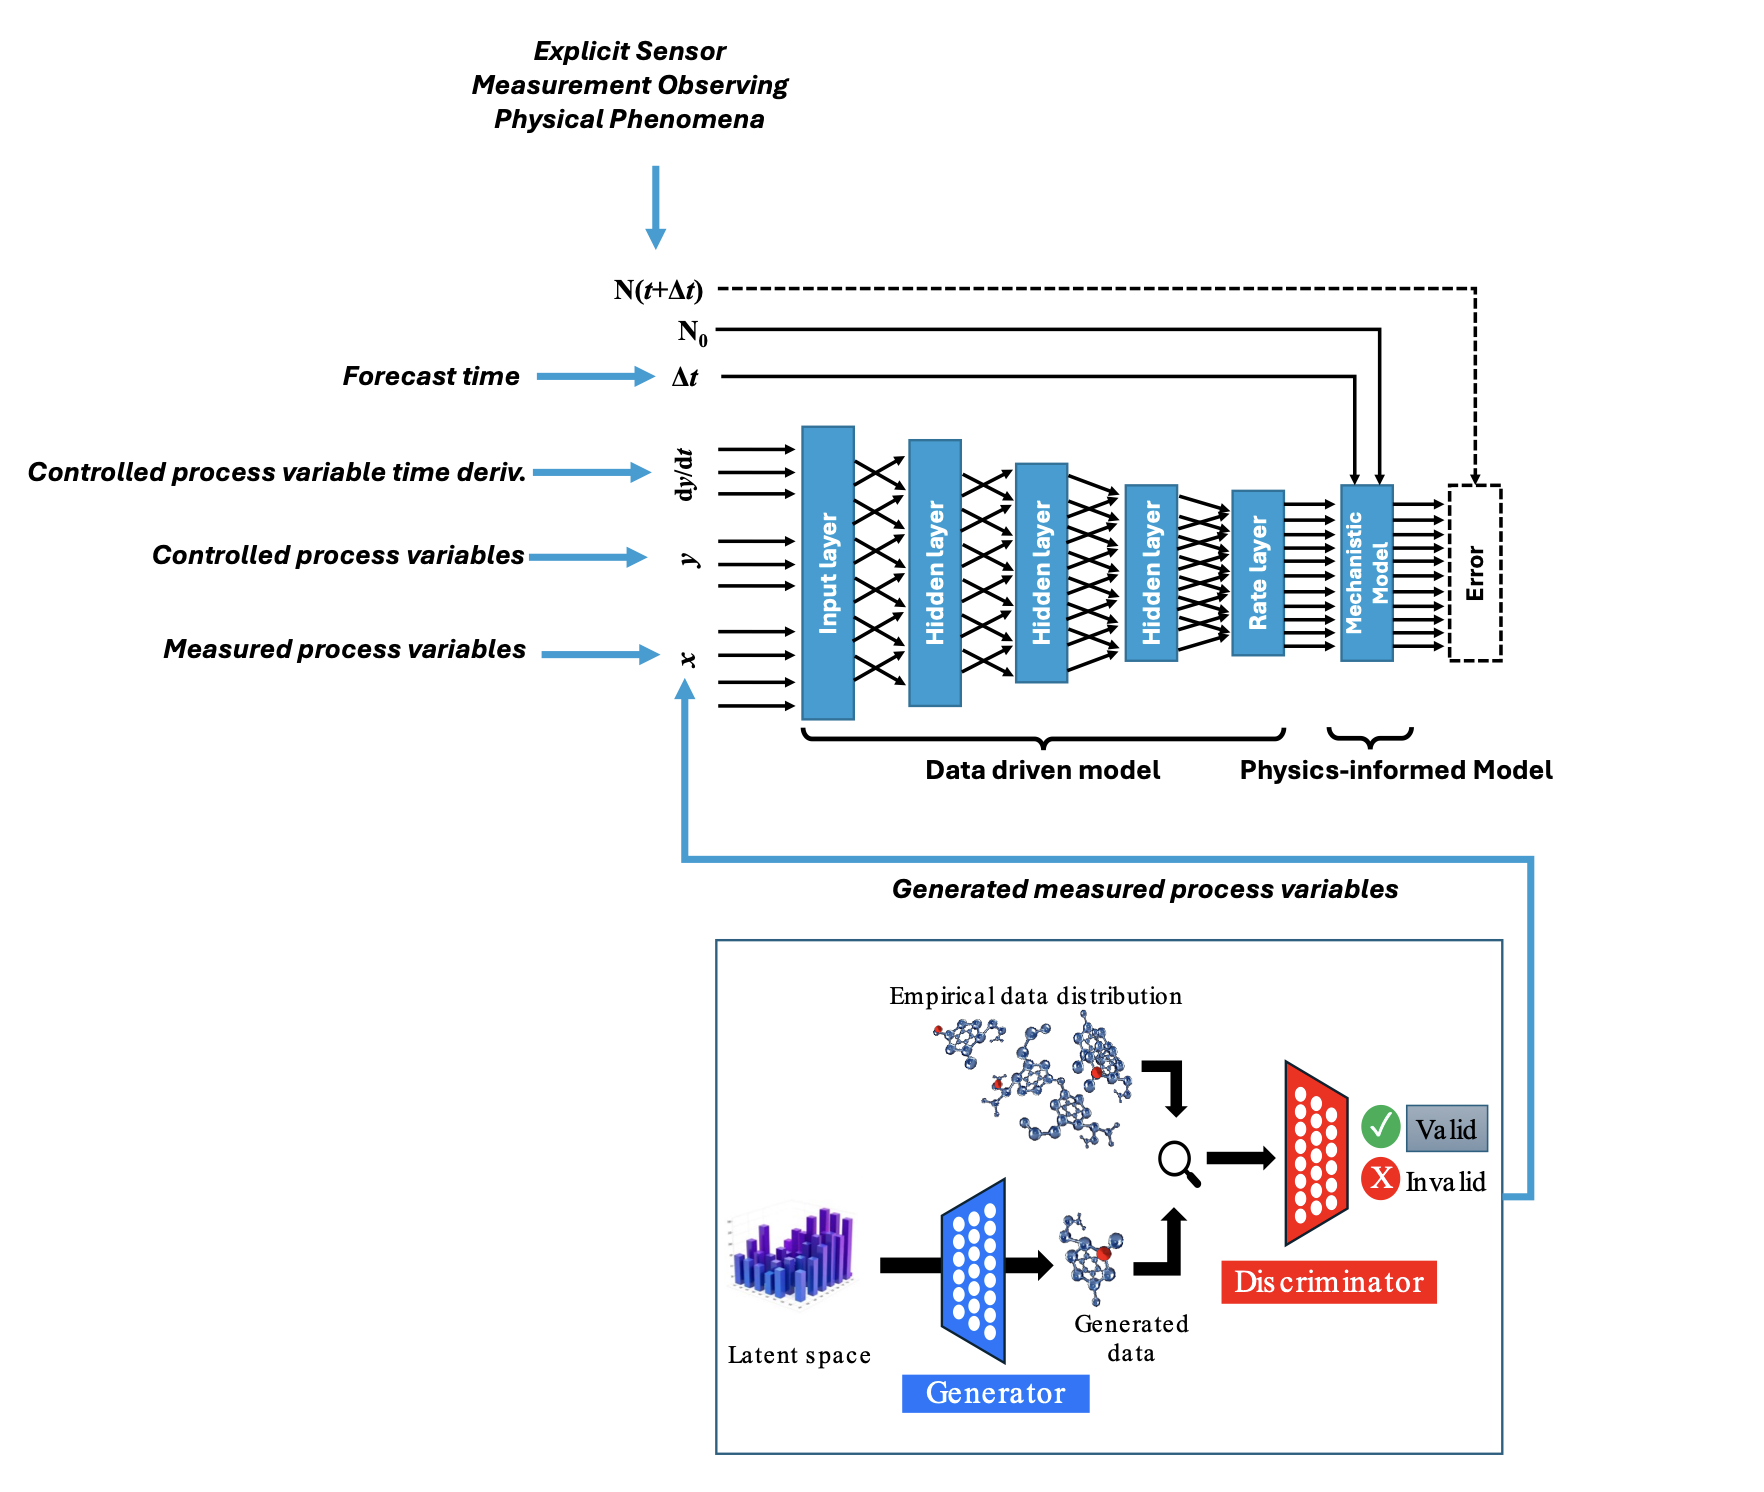
\includegraphics[width=1\linewidth]{hybridgan.png}
    \caption{QGAN and synthetic data implementation within a hybrid-model approach to process monitoring.}\label{fig:qgan_hybrid_approach}
\end{figure*}

Hybrid modeling typically combines parametric models derived from first-principles knowledge such as reaction kinetics or mass balances with nonparametric, data-driven techniques like neural networks to mitigate the challenges of sparse datasets. \cite{sharma2022hybrid} For example, hybrid models augment mechanistic simulations with machine learning to improve accuracy in bioprocessing, where experimental data are often costly and scarce due to lack of process analytical technology (PAT) or regulatory restrictions (especially in biopharmaceutical production processes), enabling reliable predictions for process optimization and control.\cite{O'Brien2021A}

The Hybrid-GAN structure integrates GANs with physics-informed mechanistic components:

\begin{equation}
\begin{split}
\min_G \max_D \bigl[ & \mathbb{E}_{x\sim p_{data}}[\log D(x)] \\
& + \mathbb{E}_{z\sim p_z}[\log(1-D(G(z)))] \\
& + \lambda\mathbb{E}_{z\sim p_z}\biggl[\biggl\|\frac{d}{dt}M(G(z)) \\
& \qquad - f(M(G(z)), t, \theta)\biggr\|^2\biggr] \bigr]
\end{split}
\end{equation}

\paragraph{Relationship to the trained objective.} The objective above is
written in the original (log-GAN / Jensen--Shannon) form,
$\mathbb{E}[\log D(x)] + \mathbb{E}[\log(1-D(G(z)))]$, augmented with a
mechanistic-residual penalty. This is deliberately distinct from the objective
actually trained in this study, which is the Wasserstein GAN with gradient
penalty (Eq.~\ref{eq:wgangp}, Earth-Mover formulation). The log-GAN form is
retained here only because it most transparently exposes where a mechanistic
residual term would attach; any future implementation of this proposed
extension would substitute the Wasserstein--gradient-penalty critic used
throughout the present work (Section~3) for the $\log D$ discriminator, so that
the Hybrid-GAN inherits the training stability documented for the deployed
QWGAN-GP rather than the mode-collapse and vanishing-gradient pathologies of
the original GAN objective.

\textbf{Components:}
\begin{itemize}[nosep, leftmargin=*]
  \item $G$: Generator mapping latent variables $z$ to generated process variables
  \item $D$: Discriminator assessing authenticity
  \item $M$: Mechanistic operator projecting generated data onto physical states
  \item $f$: Governing dynamics (e.g., ODEs describing bioprocess kinetics)
  \item $\lambda$: Weighting hyperparameter balancing data fidelity and physical consistency
  \item $\theta$: Model parameters from constitutive equations (reaction kinetics, particle size distribution, growth rates, etc.)
\end{itemize}

This optimization balances statistical fidelity from empirical data distributions ($p_{data}$) with physical consistency, minimizing residuals from time derivatives.

\subsubsection{Integration with Process Models}


\begin{figure}[ht]
  \centering
  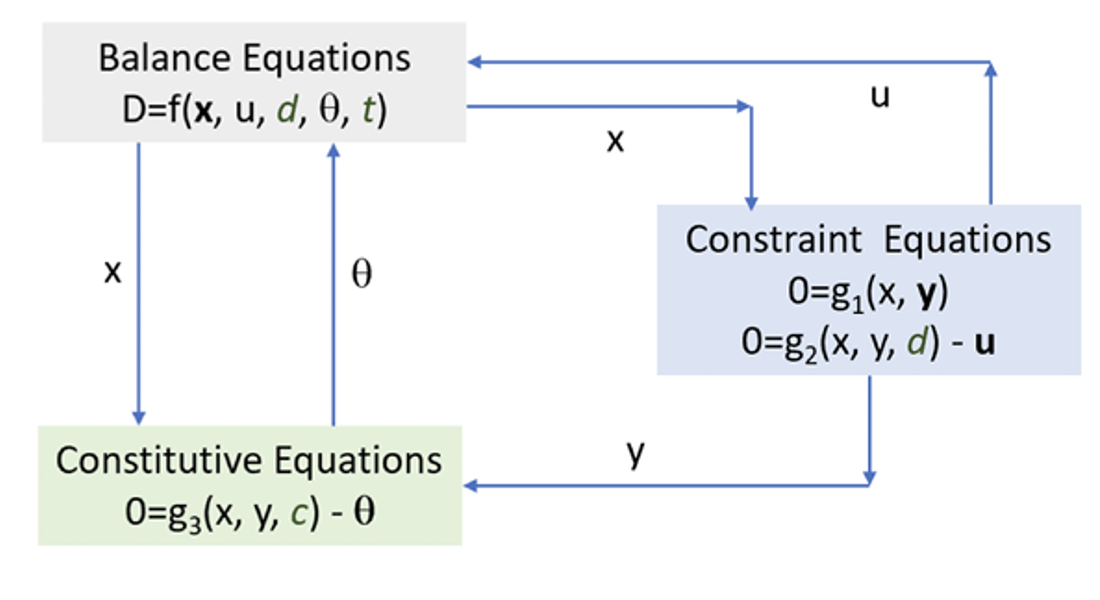
\includegraphics[width=\columnwidth]{mech_rep.png}
  \caption{Mechanistic representation of (bio)chemical processes. Reprinted with permission from Elsevier. \cite{mansouri2025models}}
  \label{fig:mech_rep}
\end{figure}

The mechanistic representation involves several key equation types:

\textbf{Balance Equations:}
\begin{equation}
  D = f(x, u, d, \theta, t)
  \label{eq:balance}
\end{equation}

\textbf{Constraint Equations:}
\begin{align}
  0 &= g_1(x, y) \label{eq:constraint1} \\
  0 &= g_2(x, y, d) - u \label{eq:constraint2}
\end{align}

\textbf{Constitutive Equations:}
\begin{equation}
  0 = g_3(x, y, c) - \theta
  \label{eq:constitutive}
\end{equation}

\noindent where:
\begin{itemize}[nosep, leftmargin=*]
  \item $c$: vector of model parameters
  \item $d$: vector of specified variables
  \item $t$: independent variable (time)
  \item $u$: vector of design variables
  \item $x$: vector of process variables
  \item $y$: vector of measured variables
  \item $\theta$: vector of physico-chemical properties
\end{itemize}

This structure extends physics-informed neural networks (PINNs) paradigm by incorporating adversarial training for synthetic data augmentation in data-limited scenarios. This connection underscores the Hybrid-GAN's utility in addressing small data challenges, where pure data-driven models fail due to insufficient training samples, by infusing prior scientific knowledge to produce robust, generalizable predictive models.

\subsubsection{Comparison with Other Modeling Approaches}

\begin{table}
\small
\caption{\emph{Qualitative, aspirational} comparison of modelling approaches in data-scarce environments. The ratings are conceptual expectations from the literature, \emph{not} measured outcomes of this study; in particular the ``Hybrid-GAN (Proposed)'' row describes a proposed architecture that was not implemented or evaluated here.}
\label{tbl:various_approaches}
\resizebox{\columnwidth}{!}{%
\begin{tabular}{p{2cm}p{2cm}p{2cm}p{2cm}p{2.55cm}p{2cm}}
\hline
\textbf{Method} & \textbf{Data Efficiency} & \textbf{Physical Consistency} & \textbf{Generative Capability} & \textbf{Interpretability} & \textbf{Robust to Small Data}\\
\hline
Pure Data-Driven Models & \textbf{\ding{55}}& \textbf{\ding{55}}& \textbf{\ding{51}}& \textbf{\ding{55}}& \textbf{\ding{55}} \\
\midrule
Mechanistic Models & \textbf{\ding{51}}& \textbf{\ding{51}}& \textbf{\ding{55}}& \textbf{\ding{51}}& \textbf{\ding{51}}\\
\midrule
Hybrid Models (Mech + ML) & \textbf{\ding{51}}& \textbf{\ding{51}}& \textbf{\ding{55}}& \textbf{\ding{51}}& \textbf{\ding{51}}\\
\midrule
PINNs & \textbf{\ding{51}}& \textbf{\ding{51}}& \textbf{\ding{55}}& \textbf{\ding{51}}& \textbf{\ding{51}}\\
\midrule
Standard GANs & \textbf{\ding{55}}& \textbf{\ding{55}}& \textbf{\ding{51}}& \textbf{\ding{55}}& \textbf{\ding{55}}\\
\midrule
Hybrid-GAN (Proposed) & \textbf{\ding{51}}& \textbf{\ding{51}}& \textbf{\ding{51}}& \textbf{\ding{51}}& \textbf{\ding{51}} \\
\bottomrule
\end{tabular}}
%}
\end{table}

This table is an \emph{aspirational} qualitative comparison: the ``Hybrid-GAN (Proposed)'' row reflects expected properties of the proposed extension and was \emph{not} experimentally validated in this study. It is provided to motivate future work, not as a demonstrated result. If a measured comparison cannot be provided, the row (or the table) may be removed at the editor's discretion.

\subsubsection{Expected Regularization Properties}

In principle, the physics term $M(G(z))$ would impose mechanistic constraints that reduce overfitting \cite{rice2020overfittingadversariallyrobustdeep}, while sensor measurements ($y$) would constrain the latent space to physically feasible dynamics \cite{hermann2025hybrid}. These properties remain to be validated empirically.


\subsection{Additional Validation Metrics Discussion} 

\subsubsection{Dynamic Time Warping (DTW) Implementation}

Dynamic Time Warping (DTW) represents a powerful technique for measuring similarity between temporal sequences that may exhibit varying lengths or temporal misalignments. \cite{dimoudis2023utilizing} The DTW algorithm operates by identifying an optimal warping path that minimizes the cumulative distance between corresponding elements of two time series while respecting monotonicity and boundary constraints.

\begin{algorithm}[ht]
  \caption{Dynamic Time Warping}
  \label{alg:dtw}
  \begin{algorithmic}[1]
    \Require Time series $S$ of length $n$, time series $T$ of length $m$
    \Ensure DTW distance between $S$ and $T$
    \State $\mathbf{DTW} \gets (n+1) \times (m+1)$ matrix
    \State $\mathbf{DTW}[0,\,0] \gets 0$
    \For{$i = 1$ to $n$}
      \State $\mathbf{DTW}[i,\,0] \gets \infty$
    \EndFor
    \For{$j = 1$ to $m$}
      \State $\mathbf{DTW}[0,\,j] \gets \infty$
    \EndFor
    \For{$i = 1$ to $n$}
      \For{$j = 1$ to $m$}
        \State $\text{cost} \gets |S[i] - T[j]|$
        \State $\mathbf{DTW}[i,\,j] \gets \text{cost} + \min\begin{cases}
          \mathbf{DTW}[i-1,\,j]   & \text{insertion} \\
          \mathbf{DTW}[i,\,j-1]   & \text{deletion} \\
          \mathbf{DTW}[i-1,\,j-1] & \text{match}
        \end{cases}$
      \EndFor
    \EndFor
    \State \Return $\mathbf{DTW}[n,\,m]$
  \end{algorithmic}
\end{algorithm}

\textbf{Interpretation:}
Lower DTW scores indicate better temporal alignment. Under the matched parameter budget and matched 2000-epoch training contract, the OD-scale DTW distance for the 55-parameter IQP:SEL quantum generator is approximately 0.30 (mean over 5 seeds). A frozen pre-v1.0 best-case checkpoint reported a DTW score of 0.6843; this value is not re-emitted under the matched-budget contract and is retained here only as a historical reference. DTW is robust to phase shifts and speed variations in time series.

\paragraph{Reconciliation with the pre-v1.0 DTW reference.}
An earlier frozen pre-v1.0 best-case checkpoint reported an OD-scale DTW distance of 0.6843. That value was computed under a legacy preprocessing pipeline (Pipeline~A; not the matched-budget Pipeline~B), under a single-seed best-case selection, and at a different epoch budget. Under the matched-budget contract (Pipeline~B, 5-seed mean, 2000 epochs) reported in Section~4 of the main text, the corresponding OD-scale DTW for the 55-parameter IQP:SEL quantum generator is $0.302 \pm 0.030$; the 0.6843 figure is retained only for historical traceability and is not directly comparable to the matched-budget results.

The selection of DTW for temporal sequence comparison stems from its ability to accommodate local temporal distortions while preserving the overall sequential structure. Unlike rigid distance metrics, DTW provides robust similarity measurements for time-dependent data by dynamically adjusting for speed variations, length differences, and localized temporal shifts that commonly occur in real-world temporal patterns.


\subsection{Code and Data Availability}
Complete code repository: \url{https://github.com/shawngibford/qgan}

Archived snapshot of the tagged release: Zenodo, DOI: \texttt{ZENODO-DOI-PLACEHOLDER} (to be assigned at release-freeze time).

The complete code, trained models, and datasets have been released for transparency, independent verification, and acceleration of subsequent advances in quantum-enhanced chemical and biochemical engineering.


\textbf{Quantum Circuit Specifications:}

The quantum circuit employs a dual-stage encoding strategy as described in Section~3 of the main text:
\begin{itemize}[nosep, leftmargin=*]
  \item 5 qubits arranged in three layers
  \item IQP (Instantaneous Quantum Polynomial) encoding
  \item Strongly entangling layers with $\text{Rot}(\phi, \theta, \omega)$ gates
  \item Range-based CNOT gates: $r = (\text{layer} \bmod (n_{\text{qubits}} - 1)) + 1$
  \item Enhanced Pauli measurements ($X$ and $Z$ expectation values)
  \item Total parameters: 55 (5 for IQP encoding, 45 for the three strongly entangling layers, 5 for measurement-preparation rotations)
\end{itemize}

\subsection{Additional Figures}

\textbf{Detailed Quantum Circuit Decomposition}


\begin{figure*}
    \centering
    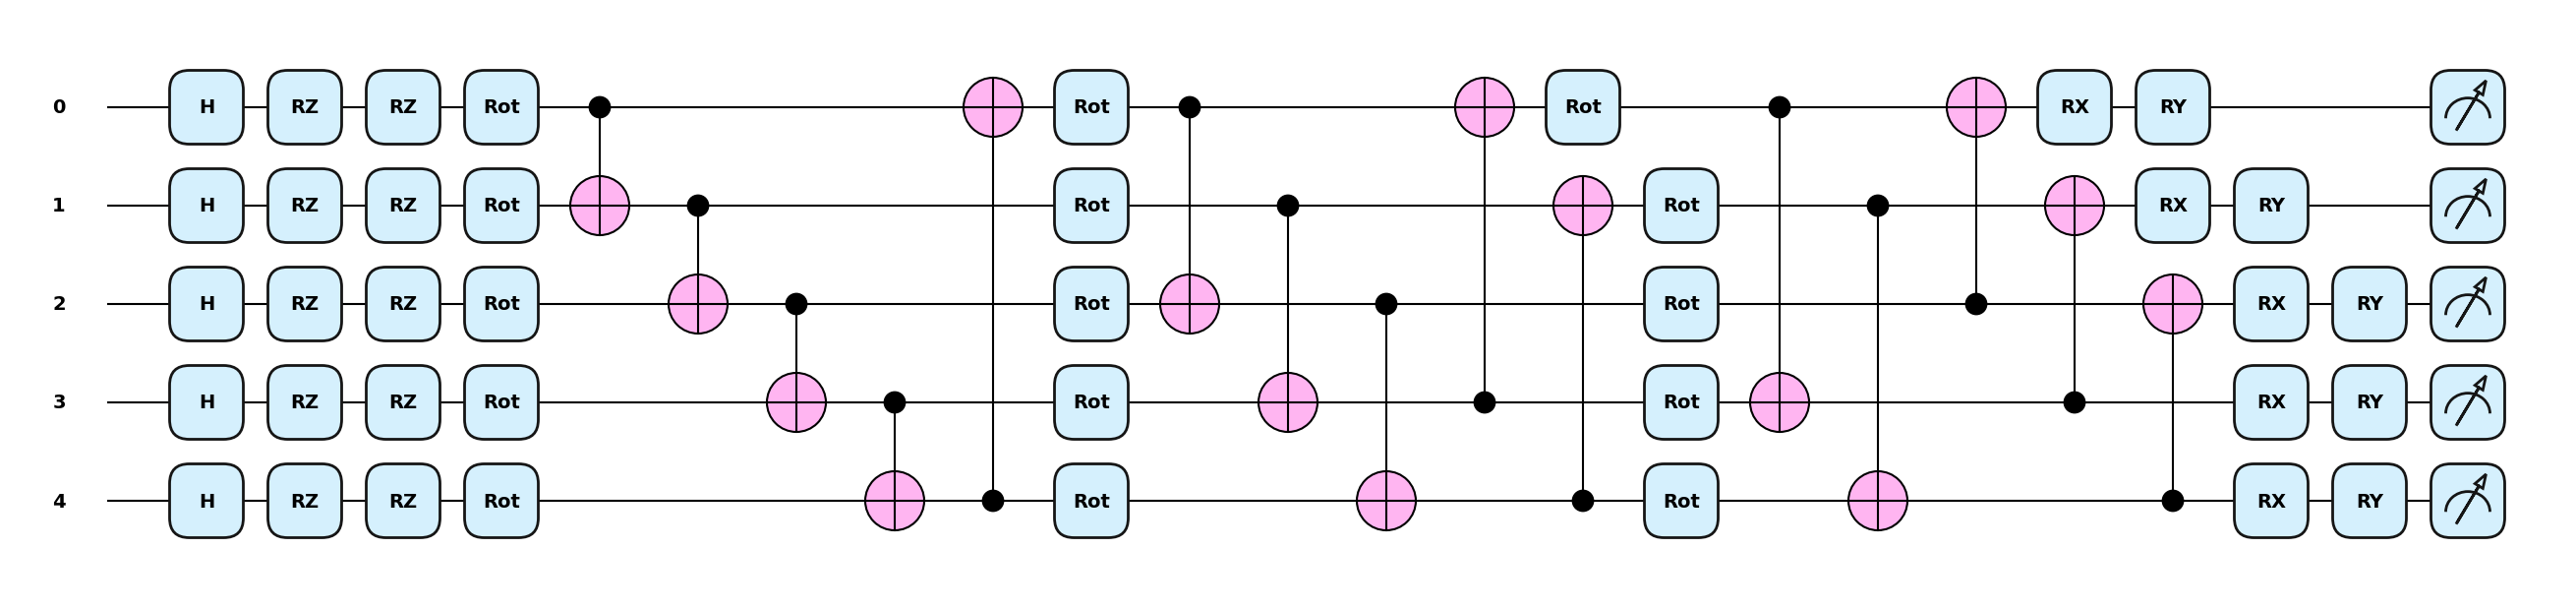
\includegraphics[height = 5cm, width=1\linewidth]{quantum_circuit.png}
    \caption{Quantum circuit used as generator.}
    \label{fig:quantum_circuit}
\end{figure*}


This figure shows the individual gate operations, including:
Hadamard gates applied to all qubits for superposition creation, 
First IQP encoding layer with Rz gates using random noise, 
Second IQP encoding layer with parameterized Rz rotations, 
Two strongly entangling layers with Rot gates and range-based CNOT gates, 
Final rotation gates (Rx and Ry) for measurement preparation, 
and Pauli-X and Pauli-Z measurements.

The circuit implements the architecture described in Section 3, leveraging quantum superposition and entanglement to explore multiple solution paths simultaneously during training, potentially affecting training dynamics (not evaluated in this study). \cite{romero2019variationalquantumgeneratorsgenerative, Amin_2018}


\begin{figure*}
    \centering
    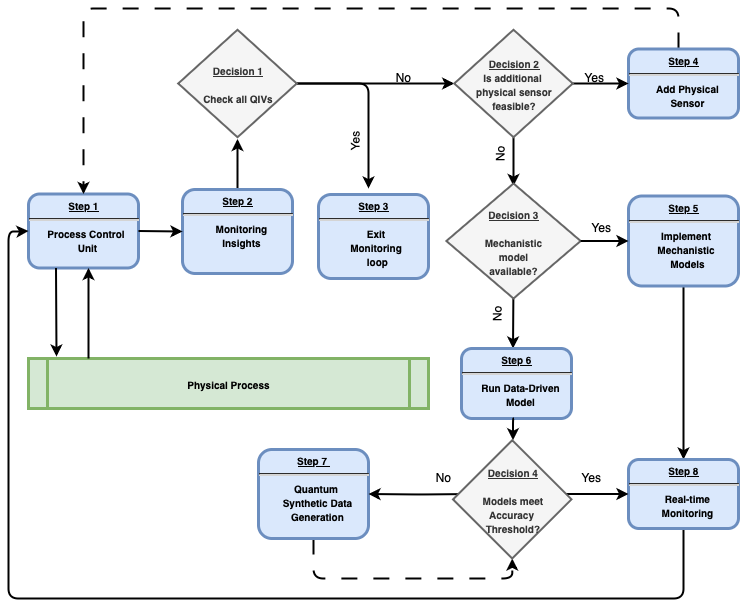
\includegraphics[width=0.75\linewidth]{bpm_qgan.drawio.png}
    \caption{Decision-tree triage schematic for bioprocess monitoring, outlined as future work in §4.5 Outlook of the main text. Not an empirical contribution of the present study.}\label{fig:qgan_schematic}
\end{figure*}
This figure illustrates the decision-tree triage workflow outlined as future work in Section~4.5 (Outlook) of the main text, sketching how sensor-feasibility, mechanistic, data-driven, and quantum-synthetic options could be organised under varying data-availability constraints. It is presented as an organising concept and is not evaluated empirically in this paper.
\begin{figure*}
    \centering
    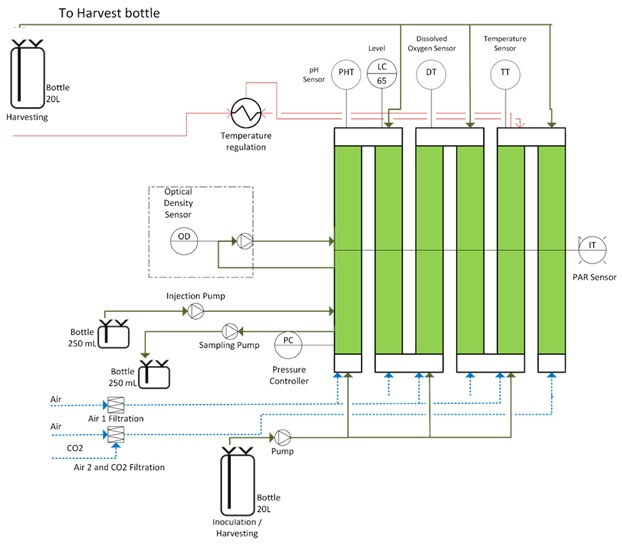
\includegraphics[width=1\linewidth]{lucy_diagram.jpg}
    \caption{Schematic of the 20\,L LUCY\textregistered{} photobioreactor used in this study, with its sensors and actuators.}
    \label{fig:lucy}
\end{figure*}

This schematic depicts the photobioreactor experimental setup described in Section~3.2, showing the sensor and actuator configuration used for data acquisition.

\subsection{Data Transformation Details}

\begin{figure}[h]
  \centering
  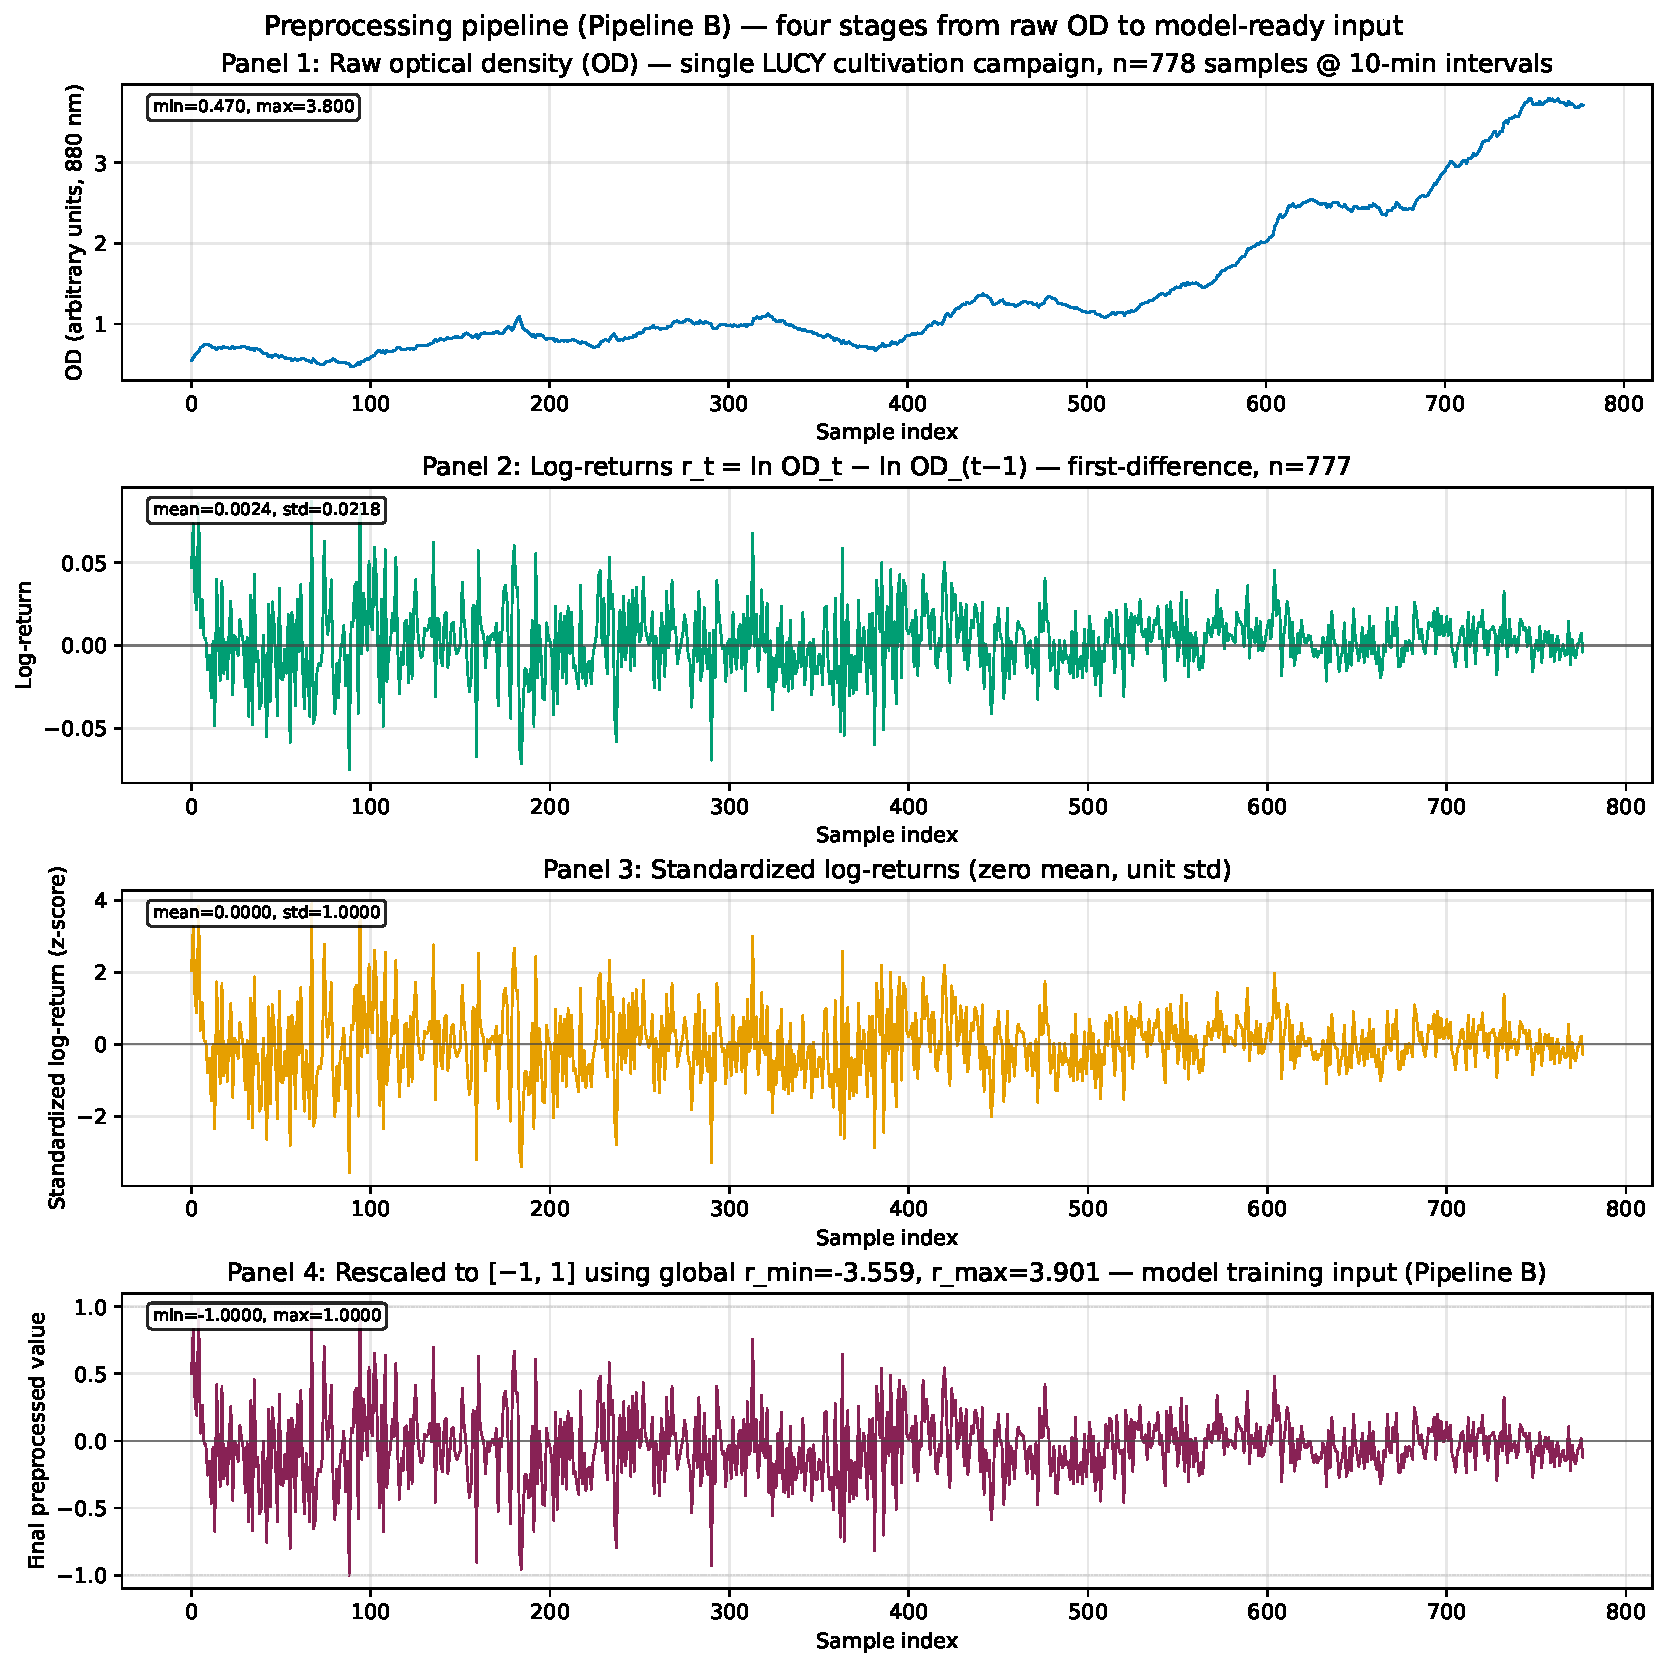
\includegraphics[width=\columnwidth]{revision/results/figures/preprocessing_pipeline_4panel.pdf}
  \caption{Four-stage preprocessing pipeline (Pipeline~B, native): raw OD ($n=778$),
  log-returns $r_t = \ln \mathrm{OD}_t - \ln \mathrm{OD}_{t-1}$ ($n=777$),
  standardized ($\mu=0$, $\sigma=1$), and inverse Lambert~$W$ heavy-tail correction
  $+$ rescale to $[-1, 1]$. The trained generators operate on the final-stage
  rescaled log-return windows; all matched-budget evaluation results in
  Section~4 of the main text are reported under this pipeline. Source:
  \texttt{revision/results/figures/preprocessing\_pipeline\_4panel.json}.}
  \label{fig:preprocessing_pipeline}
\end{figure}

The transformation from optical density measurements to log differences is motivated by the bioprocess itself: for an exponentially growing culture the optical density follows $\mathrm{OD}_t \approx \mathrm{OD}_0\,e^{\mu t}$, so the log difference between successive samples is a direct discrete estimate of the instantaneous specific growth rate. For optical density measurements $OD_t$ at time $t$:

$$r_t = \ln(\text{OD}_t) - \ln(\text{OD}_{t-1}) \;\approx\; \mu_t\,\Delta t$$

where $\mu_t$ is the local specific growth rate over the sampling interval $\Delta t$. Working in $r_t$ rather than raw OD has a direct bioprocess interpretation and three practical benefits for this growth-rate signal:
\begin{itemize}[nosep, leftmargin=*]
  \item \textbf{Growth-rate interpretability:} each $r_t$ is (up to the sampling interval) the specific growth rate, the quantity of physiological interest in cultivation monitoring, rather than an arbitrary attenuation reading
  \item \textbf{Scale/stage invariance:} the log difference is invariant to the absolute OD level, so early-exponential and high-density phases are placed on a comparable scale, which stabilises learning across the growth curve
  \item \textbf{Additivity:} growth rates over consecutive intervals sum to the net log-growth over the total span, matching how cumulative biomass increase is reported
\end{itemize}

The finance literature uses the same transform for unrelated reasons; here the justification is physiological (growth-rate estimation), not financial.

\textbf{Normalization:}
\begin{equation}
  r_t^{\,\text{NORM}} = \frac{r_t - \mu}{\sigma}
  \label{eq:normalization_s9}
\end{equation}

This brings all values to a consistent scale with mean zero and standard deviation one, which is essential for quantum circuit encoding.

\textbf{Lambert $W$ Transformation:}

The inverse Lambert $W$ transform was applied to the normalized log values to adjust for heavy tails within the distribution of the data, pushing them towards more Gaussian traits. As shown by Goerg~\cite{goerg2015lambert}, this function allows the reshaping of a distribution to align more closely with a Gaussian distribution:
\begin{equation}
  W_\delta(\nu) = \text{sgn}(\nu)\sqrt{\frac{W(\delta\nu^2)}{\delta}}
  \label{eq:lambert_w_s9}
\end{equation}

\noindent where:
\begin{itemize}[nosep, leftmargin=*]
  \item $\nu$ is a value of the dataset
  \item $\text{sgn}(\nu)$ is the sign of $\nu$
  \item $\delta$ is a programmable parameter
  \item $W$ is the Lambert $W$ function (inverse of $z = ue^u$)
\end{itemize}

This transformation is particularly important for bioprocess data, which often exhibits non-normal distributional properties due to the inherent variability and complex underlying mechanisms~\cite{boskabadi2025virtual}.

\subsubsection{Rolling Window Implementation}

Using the rolling window technique~\cite{dimoudis2023utilizing}, we generated overlapping subsequences of the original data to capture temporal patterns and dependencies. This depends on two parameters:
\begin{itemize}[nosep, leftmargin=*]
  \item \textbf{Stride ($s$):} The gap between the starts of subsequences (set to 2)
  \item \textbf{Subsequence length ($m$):} The length of each window (set to 10)
\end{itemize}

The window length ($m$) is set longer than ($s$) to guarantee enough overlap. According to Orlandi et al.~\cite{orlandi2024enhancing}, these values optimize for balanced overlap and computational efficiency. This approach is essential for capturing the temporal dependencies that characterize bioprocess dynamics, where events at one time point influence future states.

\subsection{Critic Network Architecture Details}

The Critic model is a convolutional neural network that processes sequential data to distinguish between real and generated data from the quantum generator. The network follows the WGAN-GP architecture~\cite{gulrajani2017improved} with specific adaptations for time series data.

% source: revision/results/total_adversarial_param_budget.json#shared_critic_n_params (=250881)
% source: revision/results/classical_architectures.json#models.shared_critic.total_params (=250881)
The critic network has a total of 250881 trainable parameters. This same
critic was used for all WGAN-GP generators (quantum and classical) under the
matched-budget protocol defined in main-text Section~3.1; the only component
that varies between the quantum and classical entrants is the generator,
which isolates the effect of the quantum circuit on the generated
distribution.

\textbf{Architecture Specifications:}

\textbf{Convolutional Layers:}
\begin{itemize}[nosep, leftmargin=*]
  \item Layer 1: 64 filters, kernel size 3, stride 1
  \item Layer 2: 128 filters, kernel size 3, stride 1
  \item Layer 3: 128 filters, kernel size 3, stride 1
\end{itemize}

The increasing filter count allows extraction of more complex features and produces detailed feature maps. The first convolutional layer is designed to handle input data shaped as $(10, 1)$, where the dimension of 10 represents the length of subsequences created through the rolling window approach~\cite{dimoudis2023utilizing}, ensuring the network properly processes the temporal structure of the input data.

\textbf{Activation Functions:}

Each convolutional layer is followed by a LeakyReLU activation function ($\alpha = 0.1$), which addresses the vanishing gradient issue that can cause neurons to become inactive and enables the network to learn more complex patterns through its nonlinear properties~\cite{gulrajani2017improved}.

\textbf{Dense Layers:}

Following the three convolutional layers, the data undergoes flattening to convert the multidimensional feature maps into a one-dimensional vector suitable for dense layer processing. A fully connected layer with 32 neurons is then applied with LeakyReLU activation to capture complex data relationships.

\textbf{Regularization:}

To improve generalization and reduce overfitting, a dropout layer randomly deactivates 20\% of neurons during training.

\textbf{Output Layer:}

The final output layer contains a single neuron that produces an unbounded scalar value, where higher values indicate the input resembles real data and lower values suggest generated data. This unbounded output design aligns with the use of Wasserstein distance as the cost function~\cite{arjovsky17a}, providing more meaningful gradients during training compared to the original GAN formulation~\cite{goodfellow2014generativeadversarialnetworks}.



